% Calculus and Graphs only TikZ/pgfplots setup, loaded after shared/preamble.tex
% by every sheet and answer key. Kept out of the shared preamble so this
% pillar's drawing styles cannot change how any other pillar compiles.
\usepackage{needspace}
\usetikzlibrary{calc}
\tikzset{
  cgcurve/.style={line width=0.9pt, draw=darkgray, line cap=round, line join=round},
  cgdash/.style={line width=0.5pt, dashed, draw=medgray},
  cgfill/.style={fill=gray!25, draw=none},
  cghost/.style={line width=0.5pt, dashed, draw=medgray}
}

% ── Section B4 reverse-sketching panels ───────────────────────────────────────
% Every panel is 3.6 cm tall and carries ticks at x = -2, -1, 1, 2, with the
% turning points of the question (-1 and 2) labelled. Every panel has at least
% two flat points, so the answer cannot be found by counting them. Panel D is
% correct: f'(x)=(x+1)(x-2), so f rises, flattens at x=-1, falls, flattens at
% x=2, then rises.
%
% Axes: x in [-2.5,3.35] at 0.72 cm/unit (4.2 cm wide); y in [-1.9,1.95] at
% 0.95 cm/unit (3.66 cm tall). Features are chosen to sit inside that box.
\newcommand{\cgpanelaxes}{%
  \draw[->, line width=0.5pt] (-2.5,0)--(3.35,0);
  \draw[->, line width=0.5pt] (0,-1.9)--(0,1.95);
  \foreach \tx in {-2,-1,1,2}{%
    \draw[line width=0.5pt] (\tx,-0.10)--(\tx,0.10);}%
  \node[below=1.5pt, font=\scriptsize, fill=white, inner sep=0.6pt] at (-1,0) {$-1$};
  \node[below=1.5pt, font=\scriptsize, fill=white, inner sep=0.6pt] at (2,0) {$2$};}
% A: maximum and minimum swapped: minimum at -1, maximum at 2.
\newcommand{\cgBfourA}{%
  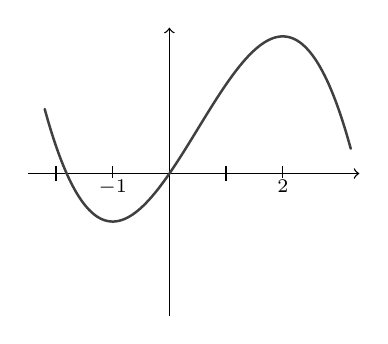
\begin{tikzpicture}[x=0.72cm, y=0.95cm]
    \clip (-2.5,-1.9) rectangle (3.35,1.95);
    \cgpanelaxes
    \draw[cgcurve, domain=-2.2:3.2, samples=200]
      plot (\x,{0.55*(-(\x*\x*\x)/3 + (\x*\x)/2 + 2*\x)});
  \end{tikzpicture}}
% B: correct +,-,+ shape but flat points at x=-2 and x=1 instead. The maximum
% sits on the -2 tick and the minimum on the 1 tick.
\newcommand{\cgBfourB}{%
  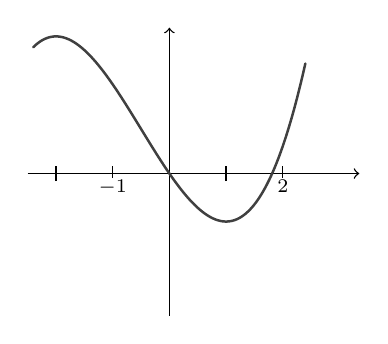
\begin{tikzpicture}[x=0.72cm, y=0.95cm]
    \clip (-2.5,-1.9) rectangle (3.35,1.95);
    \cgpanelaxes
    \draw[cgcurve, domain=-2.4:2.4, samples=200]
      plot (\x,{0.55*((\x*\x*\x)/3 + (\x*\x)/2 - 2*\x)});
  \end{tikzpicture}}
% C: flat at x=-1 where the curve does NOT turn, then a minimum at x=2.
\newcommand{\cgBfourC}{%
  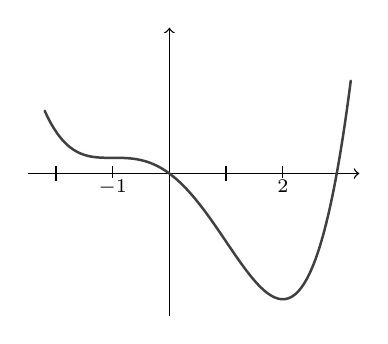
\begin{tikzpicture}[x=0.72cm, y=0.95cm]
    \clip (-2.5,-1.9) rectangle (3.35,1.95);
    \cgpanelaxes
    \draw[cgcurve, domain=-2.2:3.2, samples=200]
      plot (\x,{0.28*((\x*\x*\x*\x)/4 - 1.5*\x*\x - 2*\x)});
  \end{tikzpicture}}
% D: correct. f'(x)=(x+1)(x-2): maximum at -1, minimum at 2, then rises.
\newcommand{\cgBfourD}{%
  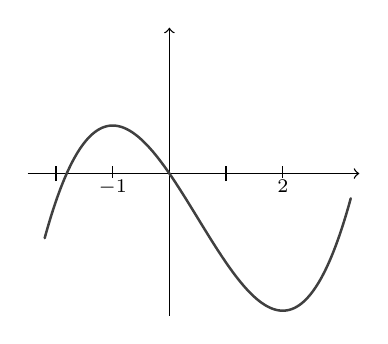
\begin{tikzpicture}[x=0.72cm, y=0.95cm]
    \clip (-2.5,-1.9) rectangle (3.35,1.95);
    \cgpanelaxes
    \draw[cgcurve, domain=-2.2:3.2, samples=200]
      plot (\x,{0.55*((\x*\x*\x)/3 - (\x*\x)/2 - 2*\x)});
  \end{tikzpicture}}
% E: maximum at x=-1, then a flat point at x=2 where the curve does NOT turn
% and keeps falling. f'(x)=-(x+1)(x-2)^2, so f' is negative on both sides of 2.
\newcommand{\cgBfourE}{%
  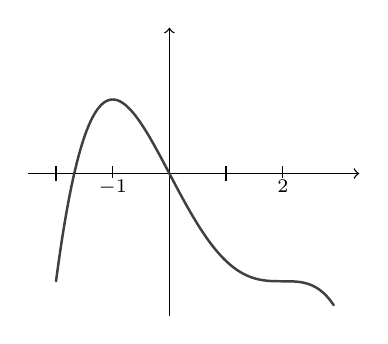
\begin{tikzpicture}[x=0.72cm, y=0.95cm]
    \clip (-2.5,-1.9) rectangle (3.35,1.95);
    \cgpanelaxes
    \draw[cgcurve, domain=-2.0:2.9, samples=200]
      plot (\x,{0.36*(-(\x*\x*\x*\x)/4 + \x*\x*\x - 4*\x)});
  \end{tikzpicture}}
